% Copyright (C) 2005-2015 Airbus - EDF - IMACS - Phimeca
% Permission is granted to copy, distribute and/or modify this document
% under the terms of the GNU Free Documentation License, Version 1.2
% or any later version published by the Free Software Foundation;
% with no Invariant Sections, no Front-Cover Texts, and no Back-Cover
% Texts.  A copy of the license is included in the section entitled "GNU
% Free Documentation License".
\renewcommand{\filename}{docUC_LowDiscrepancySequences.tex}
\renewcommand{\filetitle}{UC : Generation of low discrepancy sequences}

% \HeaderNNIILevel
\HeaderIILevel
% \HeaderIIILevel

\label{lowDiscrepancySequence}


\index{Low Discrepancy Sequences}

It is possible to generate some low discrepancy sequences in order to approximate some integrals.\\

Details on low discrepancy sequences  may be found in the Reference Guide (\extref{ReferenceGuide}{Reference Guide - Low Discrepancy Sequence}{discrepancysequence}).



OpenTURNS proposes the following sequences : Sobol, Faure, Halton, Reverse Halton and Haselgrove, in dimension $n \geq 1$.


\requirements{
  \begin{description}
  \item[$\bullet$] -
  \end{description}
}
             {
               \begin{description}
               \item[$\bullet$] a Faure sequence : {\itshape myFaureSeq}
               \item[type:] FaureSequence
               \item[$\bullet$] a Sobol sequence : {\itshape mySobolSeq}
               \item[type:] SobolSequence
               \item[$\bullet$] an Halton sequence: {\itshape myHaltonSeq}
               \item[type:] HaltonSequence
               \item[$\bullet$] an Haselgrove sequence: {\itshape myHaselgroveSeq}
               \item[type:] HaselgroveSequence
               \item[$\bullet$] a Reverse Halton sequence : {\itshape myReverseHaltonSeq}
               \item[type:] ReverseHaltonSequence
               \item[$\bullet$] the points of the sequence : {\itshape myFirstSequencePoints}
               \item[type:] NumericalSample
               \end{description}
             }

             \textspace\\
             Python  script for this UseCase :

             \begin{lstlisting}
               # Create the Faure sequence of dimension 2
               myFaureSeq = FaureSequence(2)

               # Create the Sobol sequence of dimension 2
               mySobolSeq = SobolSequence(2)

               # Create the Halton sequence of dimension 2
               myHaltonSeq = HaltonSequence(2)

               # Create the Haselgrove sequence of dimension 2
               myHaselgroveSeq = HaselgroveSequence(2)

               # Create the Inverse Halton sequence of dimension 2
               myReverseHaltonSeq = ReverseHaltonSequence(2)

               # Generate the first points of the sequence
               myFirstSequencePoints = myFaureSeq.generate(10)
             \end{lstlisting}


             To illustrate these sequences, we generate the first points (1024) from the Sobol, Halton and Reverse Halton schemes. In order to ease the comparaison with the uniformly ditributed sequence, we draw the first points obtained from the Mersenne Twister algorithm : this last sequence has a greater discrepancy than the other ones.



             \begin{figure}[H]
               \begin{minipage}{10cm}
                 \begin{center}
                   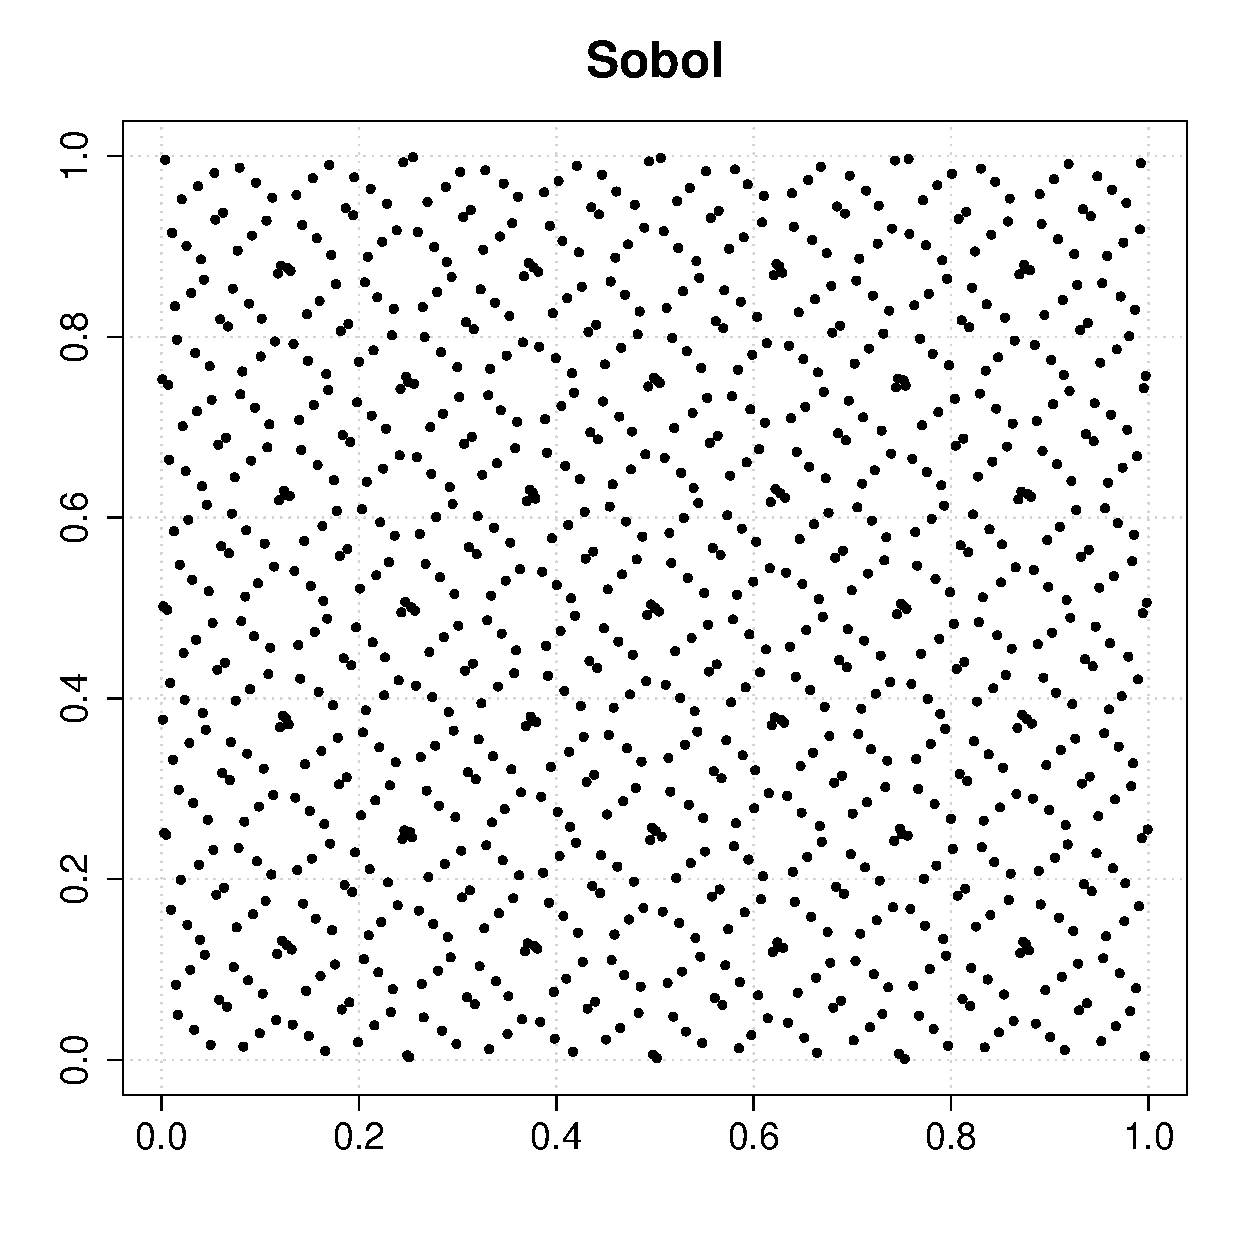
\includegraphics[width=7cm]{Figures/sobol_cloud.pdf}
                   \caption{Sobol sequence.}
                   \label{Sobol}
                 \end{center}
               \end{minipage}
               \hfill
               \begin{minipage}{10cm}
                 \begin{center}
                   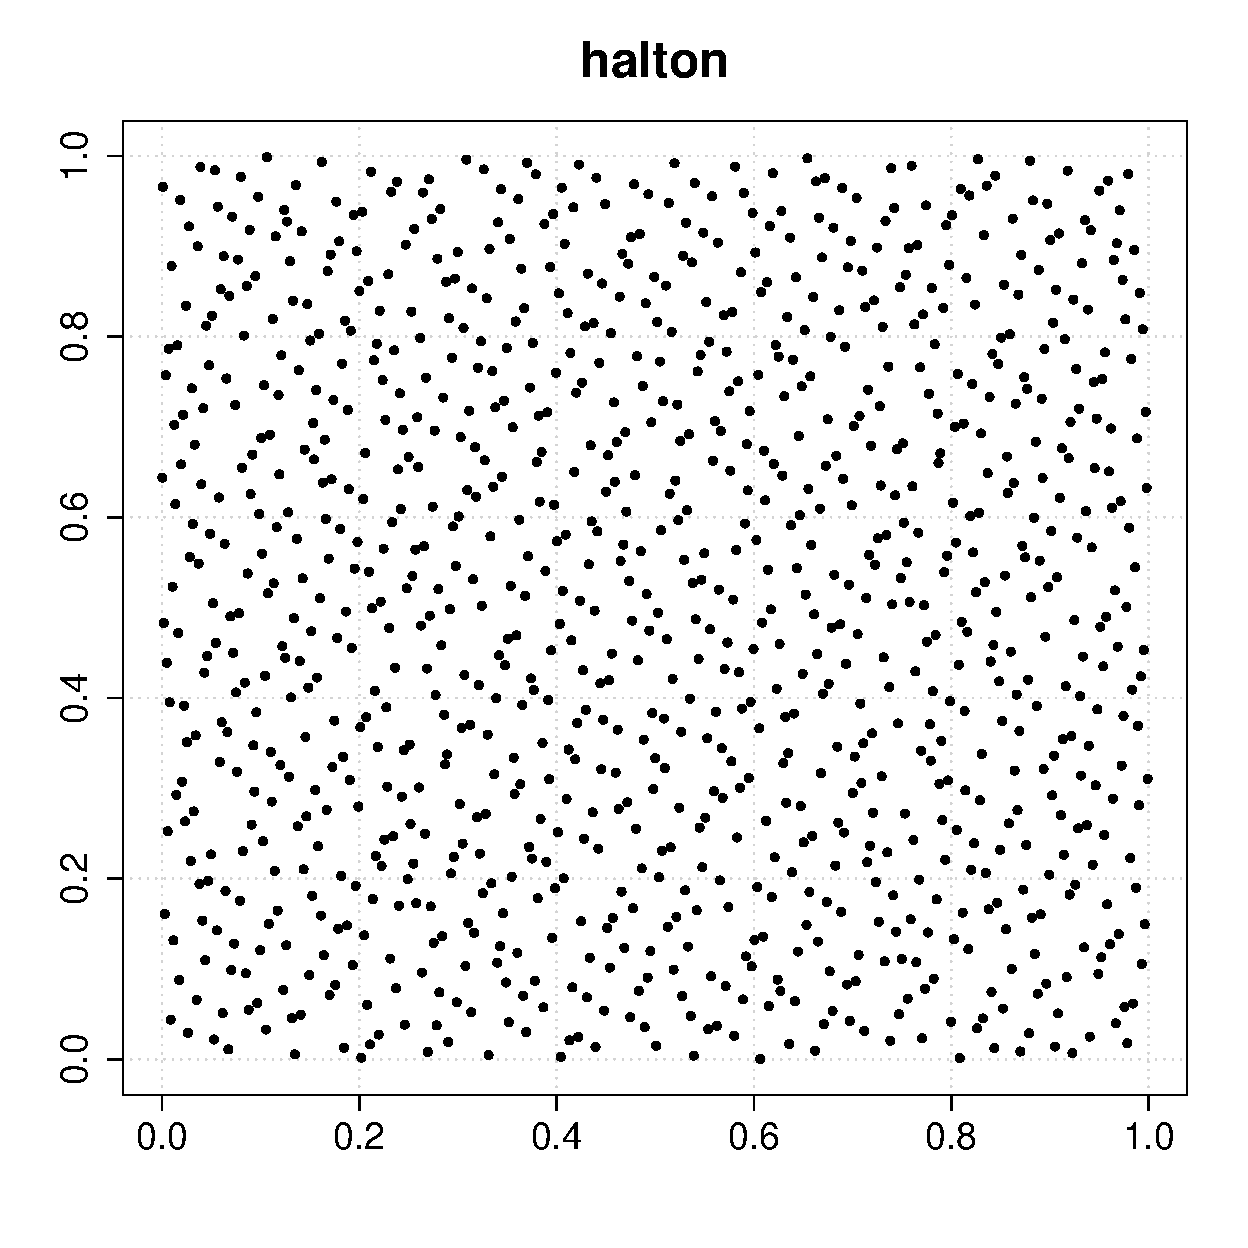
\includegraphics[width=7cm]{Figures/halton_cloud.pdf}
                   \caption{Halton sequence.}
                   \label{Halton}
                 \end{center}
               \end{minipage}
             \end{figure}


             \begin{figure}[H]
               \begin{minipage}{10cm}
                 \begin{center}
                   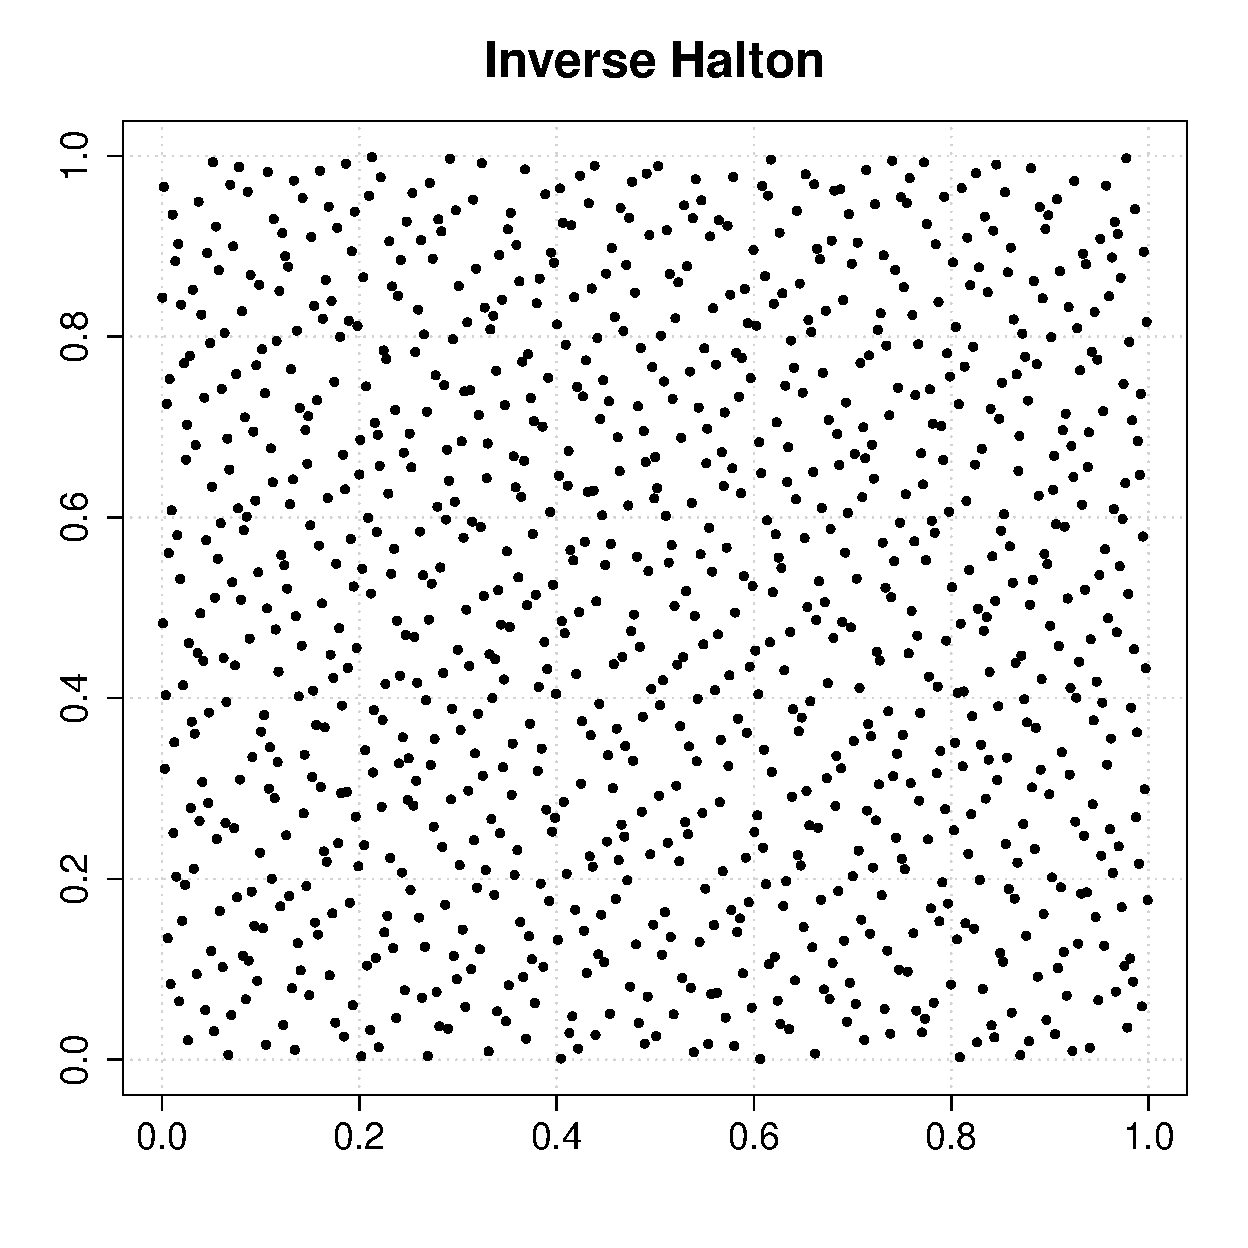
\includegraphics[width=7cm]{Figures/reverseHalton_cloud.pdf}
                   \caption{Reverse Halton sequence.}
                   \label{ReverseHalton}
                 \end{center}
               \end{minipage}
               \hfill
               \begin{minipage}{10cm}
                 \begin{center}
                   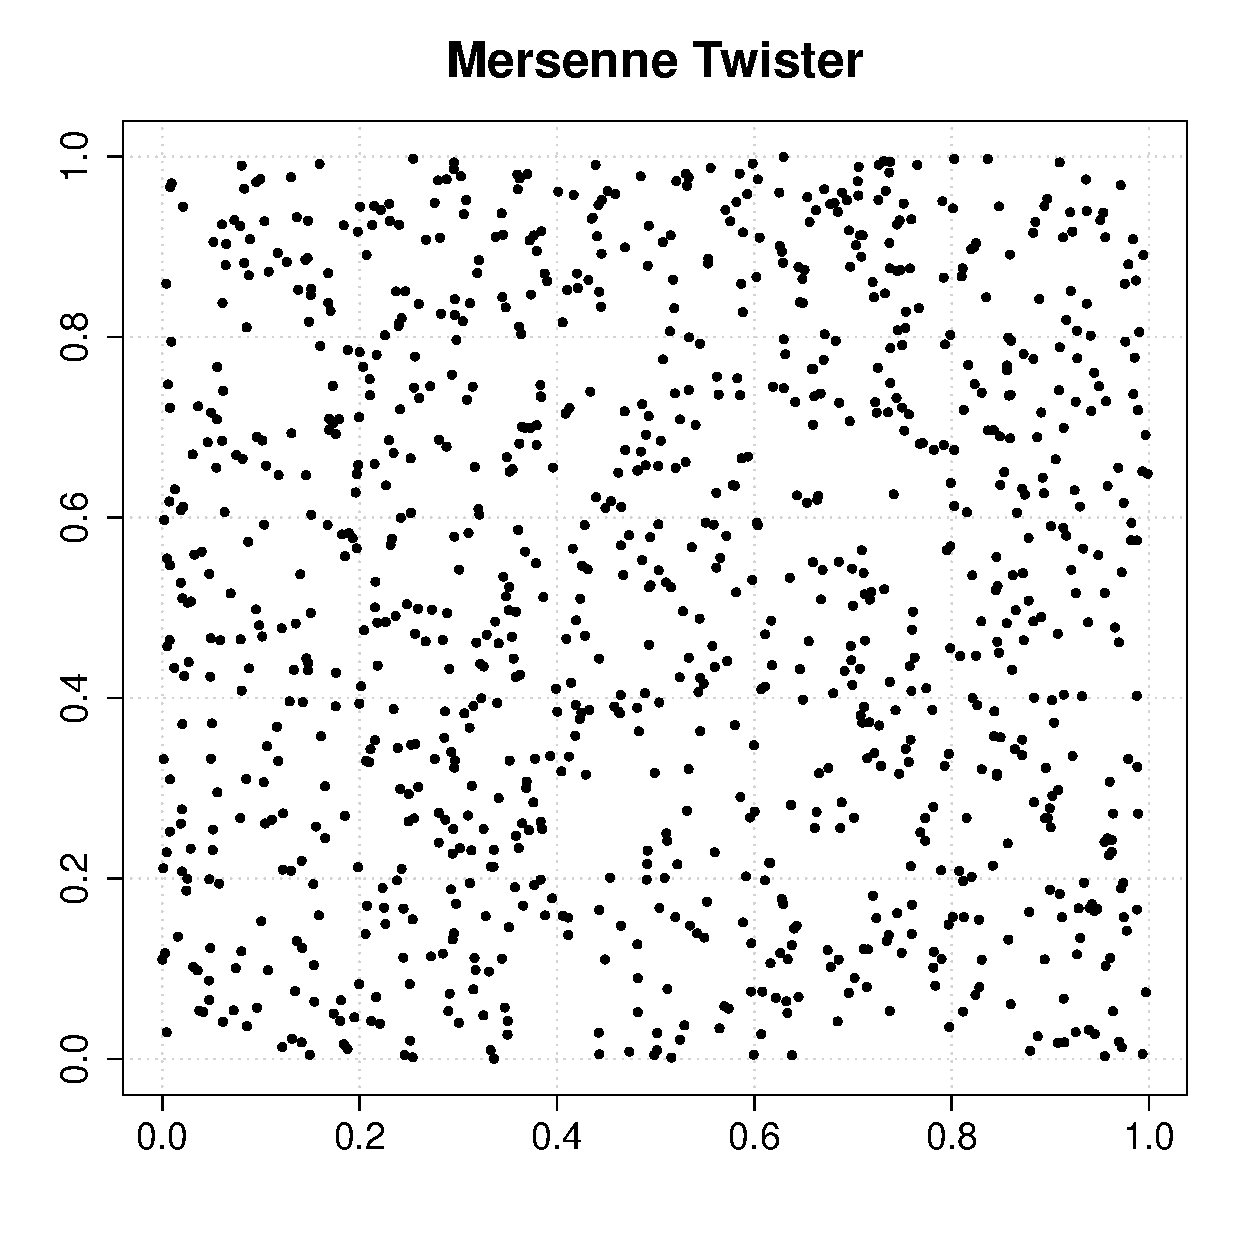
\includegraphics[width=7cm]{Figures/mersenne_twister_cloud.pdf}
                   \caption{Uniform random sequence.}
                   \label{Uniform}
                 \end{center}
               \end{minipage}
             \end{figure}
